\section{Our Method}
\label{sec:Meth}


\subsection{System Overview}
\label{subsection:overview}

\begin{figure}[!ht]
	\centering
	\includegraphics[width=3.4in]{figure/pipeline.eps}
	\caption{An overview of our layout estimation algorithm pipeline. First we adopt a multi-scale CNN achitecture \cite{eigen2015predicting} to extract geometric information from RGB images, including depth and normals. Then we combine all the abovementioned information into a multi-channel FCN , which helps to accurately estimate the layout. An optimization framwork based on perspective projection restriction is then used to generate final precise layout estimates.}
	\label{fig:pipeline}
\end{figure}

Under the Manhattan world assumption, a room layout can be represented as a cube having at most five surfaces (Three walls, Ceiling, Ground) visible in the image. 
%
Given an RGB image $\vb{I}$ with arbitrary size, our algorithm generates a room layout $\vb{L}$ consisting of a surface label for each pixel $L_{ij}\in $ $\{$Left, Front, Right, Ceiling, Ground$\}$. 
Fig. \ref{fig:pipeline} shows our algorithm pipeline. 
%%step 1
Different from \cite{dasgupta2016delay}, we first estimate depth map $D_{I}$ and normal map $N_{I}$ from the input color image to generate geometric hints using a multi-scale convolutional architecture~\cite{eigen2015predicting}, as described in Sec.~\ref{sec:depth_normal}.
%step 2
After that, to integrate information from the original RGB image together with the geometric hints, a fully convolutional network with multi-channel input is applied to predict five probability maps, each of which describes the belief for a specific layout surface, see details in Sec.~\ref{sec:surfacelabel}.
%step 3: optimization
While we can easily get access to the final layout estimation by just choose the label with highest score across the five probability maps for each pixel. 
The estimated $\vb{L}$ always have wavy boundaries and multiple disjoint connected domains due to the characteristics of neural network. To handle these problems and obtain more clear layout estimation with geometric constraints, an optimization step is adopted in Sec.~\ref{sec:optimization}.  
 

\comments{
The coarse layout estimation about semantic layout surfaces for a single RGB image, are predicted by fully convolutional neural network with geometric information emmbeded, including depth and normal information. These geometric information are estimated from source RGB image by a multi-scale convolutional architecture\cite{eigen2015predicting}. This will be decribied in Sec. \ref{subsection:CNN}. Then based on optimization framwork proposed in \cite{dasgupta2016delay}, which mainly uses perspective projection constraints, we can obtain final precise layout estimation results.
%
}


\subsection{Geometric Hints Extraction}
\label{sec:depth_normal}

We use the multi-scale convolutional network proposed in \cite{eigen2015predicting} to estimate the depth and normal map from a single RGB image, as shown in Figure~\ref{fig:depthandnormal}. Note that we do not finetune their models with our data as we do not have the depth and normals of our dataset, however, the model seems to generalize well in our case. From the global perspective, the depth and normal maps we obtained capture the overall spatial relationships between semantic surfaces. Quantitive evaluation for depth and normals extraction can be refered to in ~\cite{eigen2015predicting}.
%

\begin{figure}
	\centering
	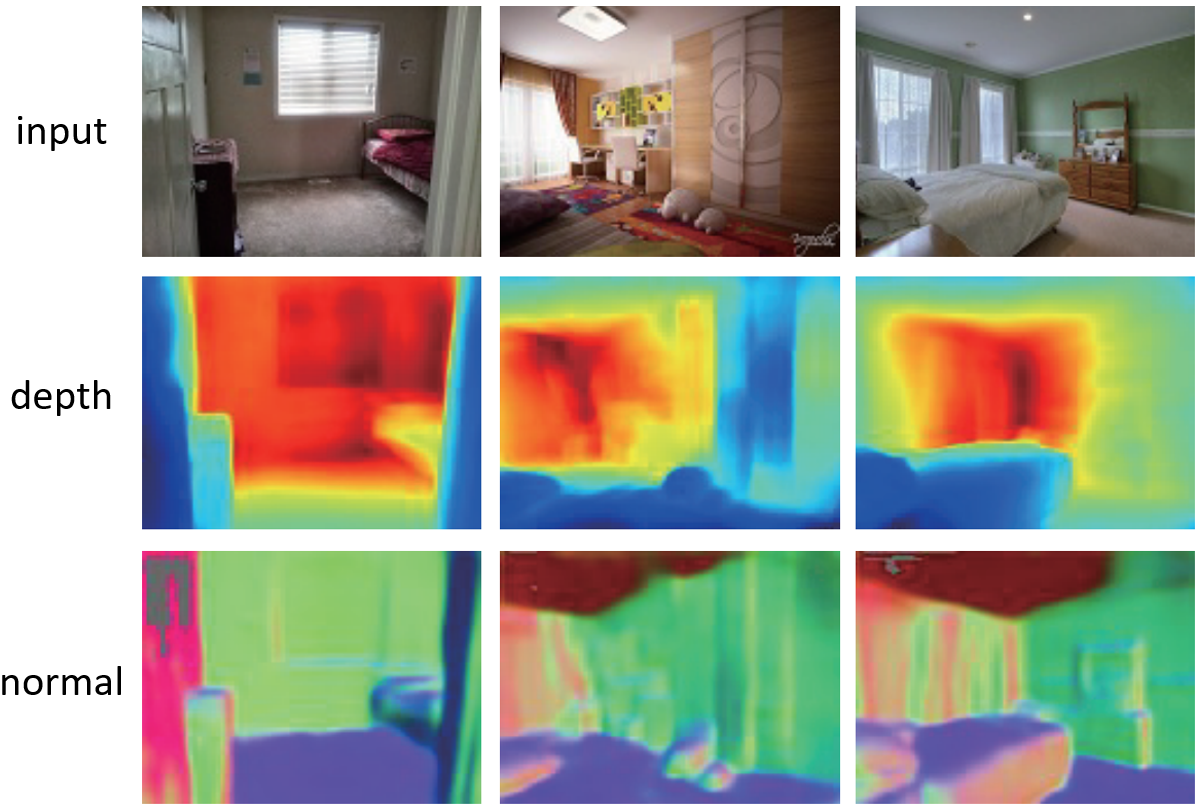
\includegraphics[width=\columnwidth]{figure/geometricinfo1.png}
	\caption{Estimation of depth and normal from a single RGB image using the multi-task FCN in \cite{eigen2015predicting}.}
	\label{fig:depthandnormal}
\end{figure}

We notice in practice that the depth maps and surface maps estimated from single RGB images are not precise in local details. And the The output resolution of the depth maps and normal maps are limited to half of the input. However, the valuable 3D information they provide is much helpful for high-level structure estimation, especially in cluttered scenes.  
%
Normals can serve as clues tending to merge big planes together, with interference factors like clutter, textures and illumination eliminated to varying degrees. 
%
These mid-level geometric information can be used to adapt and improve performance for layout estimation compared to using RGB only. 

The depth maps are color coded in \cite{eigen2015predicting} for distinction. In order to reduce the redundant information and to ensure the essence of depth, We modify their rendering section to obtain depth maps with single channel while preserving the optimization part.

\subsection{Surface Label Prediction Using MC-FCN}
\label{sec:surfacelabel}
%
In previous work, fully convolutional neural network(FCNN) or multi-task fully convolutional neural network~(MFCNN) are used to predict coarse semantic layout surfaces or layout edges \cite{dasgupta2016delay,ren2016coarse,zhao2017physics,zhang2017learning}. 
%
However, due to much clutter, complex textures and illumination variations, semantic surfaces like walls are visually separated in to pieces, making whole surfaces difficult to aggregate together. 
%
Fig.~\ref{fig:fcn-comparison}(b) shows some bad semantic surface predicting results from a widely used FCNN architecture in previous methods \cite{dasgupta2016delay,ren2016coarse}. 
The comparison between the predicted results and the ground truth reveals that due to the complex environmental factors of indoor scenes, layout results estimated from FCNN are not very reliable sometimes. 
When the occlusion happens to be at the boundaries of semantic planes, such critical clues are partially or entirely excluded, and thus we can not tell location of each plane precisely. 
Moreover, an entire plane may be predicted separately into pieces due to clutter lay in the plane.


\begin{figure}
	\centering
	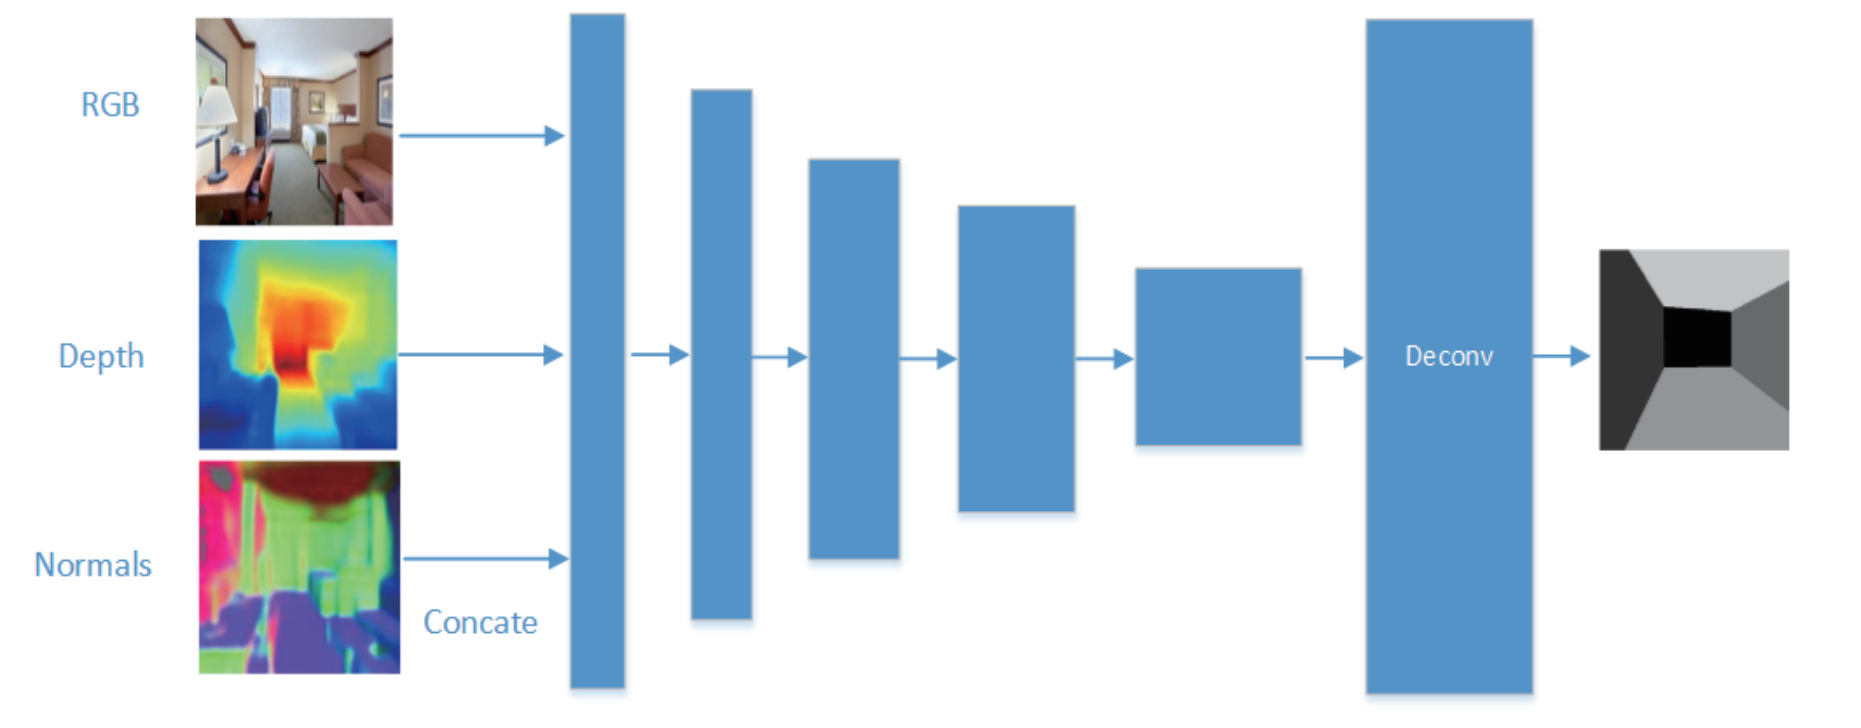
\includegraphics[width=\columnwidth]{figure/fcn-multi-channel.png}
	\caption{Illustration of the multi-channel network architecture build on \cite{chen2016deeplab}. We combine the RGB image, depth and normal together as input to the ResNet101 based FCN for semantic surface learning. }
	\label{fig:fcn-multi-channel}
\end{figure}


\textbf{Network Architecture}
To alleviate the problems caused by complex environmental factors, we fuse the geometric hints with original texture information and train a multi-channel input FCN. As Fig.~\ref{fig:fcn-multi-channel} shows, We build this multi-channel FCN on the famous architecture ResNet-101 \cite{he2016deep} modified by \cite{chen2016deeplab}. The estimated depth and normal maps are treated as additional channels associated with the input RGB images. 

\textbf{Training}
We simply concatenate different types of data to a seven-channels input(3 channels from RGB, 1 channel from depths and 3 channels from normals) which is then fed into our network. The FCN model we used for initialization from \cite{chen2016deeplab} is pretrained on MS-COCO dataset. We randomly initialize the weights for the first convolution layer to adapt to our input format and replace the weights for classifier layer with randomly initialized 5-way classifier layer. Then we specifically finetune our multi-channel FCN for semantic surface segmentation. We have also tried multi-task learning by adding a new branch for learning boundaries between surfaces as \cite{ren2016coarse, mallya2015learning} do. But the joint training doesn't help to improve the performance of both task in our case. This may indicate that our geometric hints have already integrated the additional information which should be learned through joint training.

The output of our multi-channel FCN is a $w\times h \times 5$ multidimensional array $\vb{T}$, where w and h stand for the width and length of the input rgb image. Each of the 5 slices can be viewd as a probability map for the corresponding surface label. Some visualized results compared with FCN without geometric hints as additional input are shown in Fig.~\ref{fig:fcn-comparison}. We utilize the probability array $\vb{T}$ as the basis for our scoring function. Then an optimization step based on this score function is applied to obtain precise layout estimation.


\begin{figure}[!ht]
	\centering 
	\textsc{\includegraphics[width=3.4in]{figure/fcn.eps}}
	\caption{Layout estimation results using different architectures. Row from top to bottom: (a) the input RGB image. (b) Surface predictions using the FCNN architecture used in \cite{dasgupta2016delay,ren2016coarse}. (c) our MC-FCN. (d) The ground truth. Our method generate much more clear edges, less holes.}
	\label{fig:fcn-comparison}
\end{figure}


\subsection{Layout Generation}
\label{sec:optimization}
We adopt a popular model that several researchers ~\cite{hedau2009recovering, wang2013discriminative, dasgupta2016delay, ren2016coarse} have used to parameterize indoor layout based on the Manhattan world assumption. 
Indoor scene layout is modeled as the projection of a cuboid which can be defined by 

\begin{equation}
	\label{eq:Layout}
	L = (l1, l2, l3, l4, v)
\end{equation}

where $l_{i}$ stands for $i^{th}$ line and $v$ stands for the specific vanishing point. The whole scene is equivalent to be labeled with five semantic surfaces, coresponding to \{Left, Front, Right, Ceiling, Ground\}, as described in Fig. \ref{fig:2.model}. Based on Eq. (\ref{eq:Layout}), each surface can be reconstructed with extension lines between vanishing point $v$ and Intersection point $p_i$ among $l_{i}$. ie $ve_i$ . Due to the uncertainty of camera pose, five surfaces are not always visible. Examples with different topologies are given in Fig. \ref{fig:different-layout-type}.


To obtain the optimized box layout $\vb{L}$, \cite{dasgupta2016delay} has propose a refinement algorithm. They first generate an initial $\vb{\hat{L}}$ by pick the label with the highest score across five channels of $\vb{T}$. Then a preprocessing step is used to address spurious regions and multiple disjoint components in $\vb{\hat{L}}$. Finally, an iterative optimization method is employed to acquire the refined $\vb{L}$. However, the initial $\vb{\hat{L}}$ generated from $\vb{T}$ are sometimes too ambiguous due to the characteristics of neural network. The preprocessing step can't adapt to all the bad situations well, especially when the ambiguous walls are close in size. 


To make the optimization method more general and efficient, we simplify the refinement algorithm in \cite{dasgupta2016delay} by replace the first two step with a proposing-ranking framework. Our proposing-ranking framework directly generate an initial $\vb{\hat{L}}$ that consistent with the definition in Eq.~\ref{eq:Layout}. This kind of $\vb{\hat{L}}$ are much robust to ambiguous cases and easier for the optimization step to find the refined layout.

The proposing-ranking framework is implemented by extracting enough proposals using the approach in \cite{hedau2009recovering} and a score function based on $\vb{T}$. We sample 30 rays per vanishing point to acquire enough proposals. Then we extend the modified score function in \cite{dasgupta2016delay} for special cases to adapt to all images. Given a specific label, We simply sum up the probability across 5 channels of $\vb{T}$ seperately in the same region and choose the maximum as the score for this specific label. This policy is applied just among three walls which mainly cause the ambiguity. The same extended score function is adopted in optimization step. Our postprocessing framework generalize well to ambiguous cases.

\comments{
\textbf{Preprocessing} 
Although we have more robust surface prediction result from our FCN-MC. Problems like spurious regions and multiple disjoint components are still a bit disturbing. To address these problems we simplify the preprocessing step in ~\cite{dasgupta2016delay} for efficiency. First, we address the multiple disjoint components (which means the connection domain for each label is not unique) by remove all but the largest connected domain for each label. Then we fill the holes created by this pruning with labels around them by using k-nn. After that we apply some simple contraints based on common sense to handle spurious regions.}

\begin{figure}
	\centering
	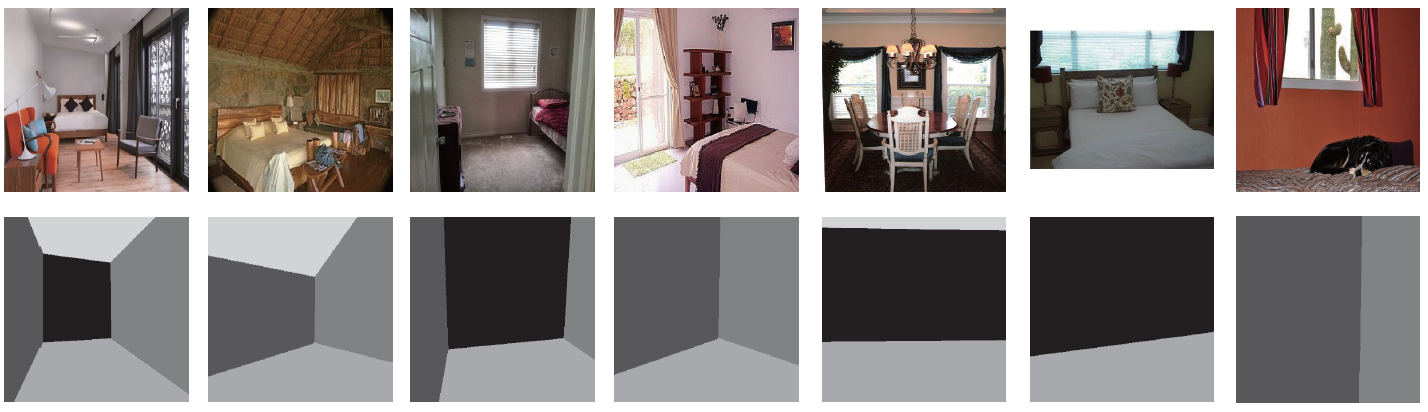
\includegraphics[width=\columnwidth]{figure/different-layout-type.png}
	\caption{Different layout type due to variation in camera pose. \drf{I'm not sure whether this situation should be discussed, so the caption is brief.} }
	\label{fig:different-layout-type}
\end{figure}